The methods of probability distribution were already explained in \textit{chapter \ref{chapter:structured_prediction}: \nameref{chapter:structured_prediction}}. This estimation is conducted separately for every feature and it is based on a training set of images. For the first type of features, which are dependent on a colour of neighbouring superpixel and its position in a grid, estimation is pretty simple. Because of the fact that each such feature is discrete, it is enough to go through the whole training set and count how many times a given colour appears in a given position. Then, by dividing this number by the total number of superpixels in all training images the probability of a given feature is obtained. For every feature, probabilities of each label are cached, and then in a training and inference processes conditional probability $p(y_i|f_i)$ can be computed straight away.

For features representing a percentage of colours in the neighbourhood of superpixels from the already described grid, the probability distribution is more difficult to obtain. Those features have continuous values and therefore it is not possible to count how many times a given value occurs in the training set. Initially in the thesis, this distribution was computed using Parzen-Rosenblatt Kernel estimation, which allowed to estimate a probability of an unknown sample for which the distribution was modelled. However, this method had one but huge drawback, as in order to obtain this estimation, it was necessary to iterate through every training sample. During the training process, in each epoch and for every superpixel in every image there was a need to compute this probability. Furthermore, while constructing a Gibbs sample the procedure had to be repeated for every label in every position in a created Markov chain. Because of this, the resources needed to for the training process were enormous, even for small datasets. Therefore, another method of probability distribution estimation had to be implemented. Similarly, as in the case of colour-position features it was necessary to choose such a method that will model this distribution only once, and give a probability of an unknown sample without a need of excessive computation. This can be obtained by means of probability histograms, in which the whole distribution is divided into a limited set of bins, and each bin is characterised by its probability of occurrence. The number of bins is the next hyperparameter of the described system. Tough the colour percentage features have continuous values, they are quite repetitive as the number of neighbouring superpixels is roughly the same and therefore, the number of histogram bins does not need to be large. 

Having constructed histograms for each feature and each label, a conditional probability of a label on a given feature can be obtained. A description of histograms that are used to calculate this probability will be explained on an example of features number 73,74 and 75. These features represent a percentage of red, green and blue neighbours of a middle superpixel, being a superpixel for which the label is to be predicted. Figure \ref{fig:nonlinear_histogram_red} shows histograms for \nth{73} feature divided into 17 bins that was constructed based on a grid of $7 \times 7$ elements and the neighbourhood size of two. The upper border value of each bin is marked on the x axis of the presented histogram. 
\begin{figure}[!htb]
    \centering
    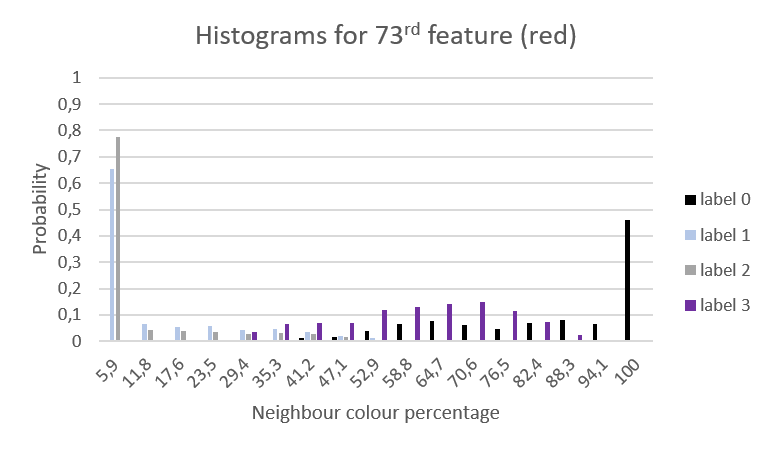
\includegraphics[width=\textwidth]{nonlinear_intro/histograms/red.png}
    \caption{Histograms for \nth{73} feature - percentage of red neighbours.}
    \label{fig:nonlinear_histogram_red}
\end{figure}
From this figure, the dependence between the colours of neighbouring superpixels and a label is clearly visible. If all neighbours are red then the most probable label for a given superpixel is 0. If not all, but the majority of superpixels are red, then either label 0 or label 3 are winning. On the other hand, if no neighbouring superpixels are red, then there is no chance of this superpixel to be classified with label 0, nor 3. The next histogram, for \nth{75} feature, is presented in Figure \ref{fig:nonlinear_histogram_green}.
\begin{figure}[!htb]
    \centering
    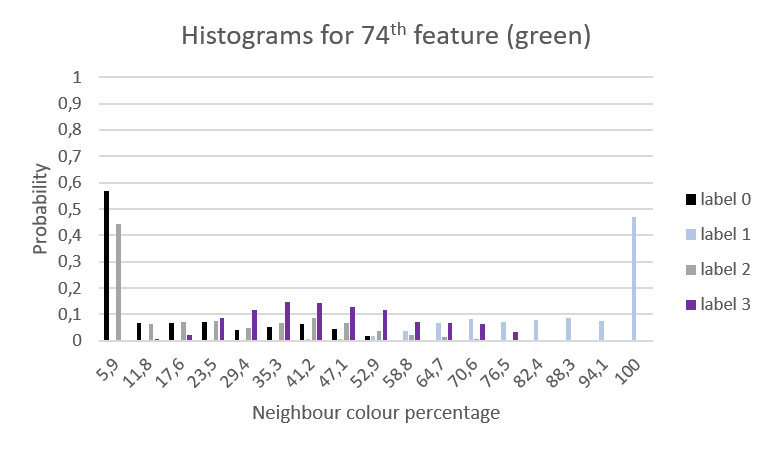
\includegraphics[width=\textwidth]{nonlinear_intro/histograms/green.png}
    \caption{Histograms for \nth{74} feature - percentage of green neighbours.}
    \label{fig:nonlinear_histogram_green}
\end{figure}
This histogram shows how green neighbours affect the label of the superpixel under consideration. If there is around 80\% or more of green neighbours than the highest probability of occurrence has the label 1. For a smaller number of green neighbours, label 3 is the most probable, however, if there are only a few green superpixels in the neighbourhood or none then the given superpixel is not a part of the object of class 3. Last histogram, presented in Figure \ref{fig:nonlinear_histogram_blue} was created for \nth{75} feature.
\begin{figure}[!htb]
    \centering
    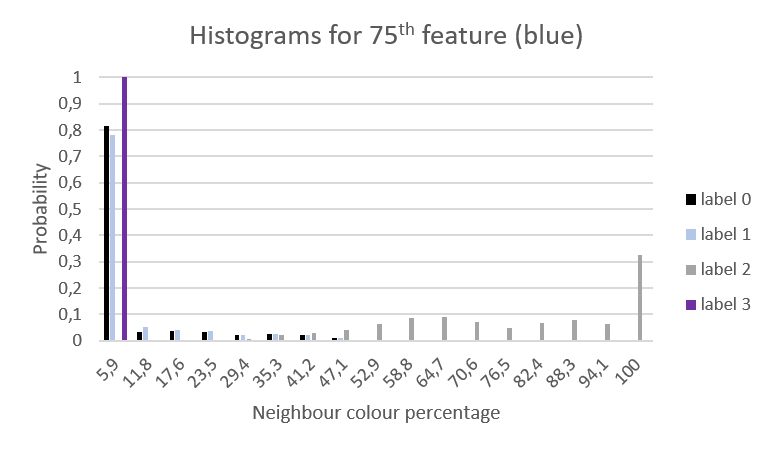
\includegraphics[width=\textwidth]{nonlinear_intro/histograms/blue.png}
    \caption{Histograms for \nth{74} feature - percentage of blue neighbours.}
    \label{fig:nonlinear_histogram_blue}
\end{figure}
From this histogram it can be read, that label 3 may be assigned to the given superpixel only if there are no blue superpixels in the neighbourhood. Even if there is only one blue neighbourhood this probability drops to 0\%, which is true because letter H is always surrounded by a green region. The bluer the neighbourhood is, the more probable is the label 2.

With the use of such histograms probability distribution for every feature and label was modelled. In order to get the probability of a given label for an unknown sample conditioned on a single feature from the chosen feature set, it is enough to check in which bin value of this feature falls and read its probability from the respective histogram. By analysing such histograms for a combination of different features it is possible for Conditional Random Fields to learn a shape of objects that are present in an image. The resulting conditional probability is an output of the feature function for the unary potential that was chosen for this part of the system.